\chapter{Hasil dan Pembahasan}

Bab ini menyajikan hasil dari seluruh tahap analisis yang telah dilakukan, dimulai dari hasil praproses data, \textit{map matching}, segmentasi trajektori, hingga analisis matriks OD, indikator intensitas persimpangan, distribusi ping per trip, dan pola OD zona eksploratif. Seluruh hasil ditafsirkan sebagai indikator kendaraan teramati berbasis MPD aktif, bukan sebagai volume lalu lintas aktual.

\section{Hasil Praproses dan Map Matching}

\subsection{Ringkasan Reduksi Data}

Pipeline praproses dimulai dari 15.386.869 titik GPS pada wilayah kajian dengan 370.778 MAID unik. Penyaringan berbasis R-tree terhadap jaringan RRU dengan ambang 20 meter menghasilkan 839.304 kandidat titik GPS. Setelah tahap \textit{bilocation collapse}, jumlah titik berkurang menjadi 552.413 titik dari 42.613 MAID. Selanjutnya, klasifikasi moda mempertahankan 236.700 titik dari 8.458 MAID yang terindikasi sebagai kendaraan bermotor. Ringkasan reduksi data ditunjukkan pada Tabel \ref{tab:hasil-reduksi}.

\begin{table}[htbp]
\centering
\caption{Ringkasan Hasil Reduksi Data}
\label{tab:hasil-reduksi}
\begin{tabular}{lrr}
\hline
Tahap & Titik GPS & MAID Unik\\
\hline
Data wilayah kajian & 15.386.869 & 370.778\\
R-tree candidates & 839.304 & 45.691\\
\textit{Bilocation collapse} & 552.413 & 42.613\\
Kendaraan bermotor terindikasi & 236.700 & 8.458\\
Trip valid hasil segmentasi & 212.407 & 8.382\\
\hline
\end{tabular}
\end{table}

Reduksi ini menunjukkan bahwa hanya sebagian kecil titik GPS pada wilayah kajian yang memenuhi kriteria kedekatan terhadap jaringan RRU dan memiliki pola gerak yang terindikasi sebagai kendaraan bermotor. Oleh karena itu, denominator hasil penelitian ini adalah kendaraan terindikasi yang teramati pada koridor RRU dalam sampel MPD aktif, bukan seluruh kendaraan yang melintas di lapangan.

\subsection{Hasil Map Matching}

Proses \textit{map matching} geometris dilakukan dengan memilih segmen jalan terdekat untuk setiap titik GPS kendaraan. Sebanyak 236.700 titik berhasil dicocokkan ke jaringan RRU. Statistik jarak pencocokan ditunjukkan pada Tabel \ref{tab:mm}.

\begin{table}[htbp]
\centering
\caption{Statistik Jarak \textit{Map Matching}}
\label{tab:mm}
\begin{tabular}{lr}
\hline
Metrik & Nilai\\
\hline
Titik GPS tercocokkan & 236.700\\
MAID unik & 8.458\\
Segmen jalan unik & 593\\
Rata-rata jarak pencocokan & 6,0 m\\
Median jarak (P50) & 5,0 m\\
Persentil 90 (P90) & 12,4 m\\
Persentil 99 (P99) & 19,2 m\\
\hline
\end{tabular}
\end{table}

Nilai median 5,0 meter dan persentil ke-99 sebesar 19,2 meter menunjukkan bahwa mayoritas titik yang lolos penyaringan R-tree berada relatif dekat terhadap jaringan jalan RRU dalam ambang yang digunakan. Namun, statistik ini dihitung setelah filter radius 20 meter, sehingga tidak dapat diperlakukan sebagai validasi independen akurasi \textit{map matching}. Hasil tersebut lebih tepat dipahami sebagai deskripsi kedekatan geometris titik yang telah lolos filter terhadap jaringan analisis.

\section{Hasil Segmentasi Trajektori}

Segmentasi trajektori dengan ambang gap 10 menit menghasilkan 38.973 trip valid dari 8.382 MAID. Statistik ringkas hasil segmentasi ditunjukkan pada Tabel \ref{tab:trip}.

\begin{table}[htbp]
\centering
\caption{Statistik Hasil Segmentasi Trajektori}
\label{tab:trip}
\begin{tabular}{lr}
\hline
Metrik & Nilai\\
\hline
Total trip & 38.973\\
Total ping dalam trip valid & 212.407\\
MAID dengan trip valid & 8.382\\
Durasi trip median & 223 detik\\
Durasi trip rata-rata & 333 detik\\
Rata-rata ping/trip & 5,45\\
Median ping/trip & 4\\
Persentil 75 ping/trip & 6\\
Persentil 90 ping/trip & 11\\
Trip dengan maksimal 5 ping & 70,37\%\\
Trip dengan minimal 10 ping & 12,88\%\\
\hline
\end{tabular}
\end{table}

Distribusi jumlah ping per trip menunjukkan bahwa data MPD aktif yang digunakan bersifat sparse. Sebanyak 70,37\% trip memiliki paling banyak 5 ping, sedangkan hanya 12,88\% trip memiliki sedikitnya 10 ping. Kondisi ini menjadi dasar penting dalam interpretasi hasil. Analisis agregat, seperti OD zona dan intensitas persimpangan, masih layak digunakan untuk deskripsi sampel MPD aktif, tetapi rekonstruksi lintasan detail dan klasifikasi belokan aktual tidak dilakukan.

\begin{figure}[htbp]
\centering
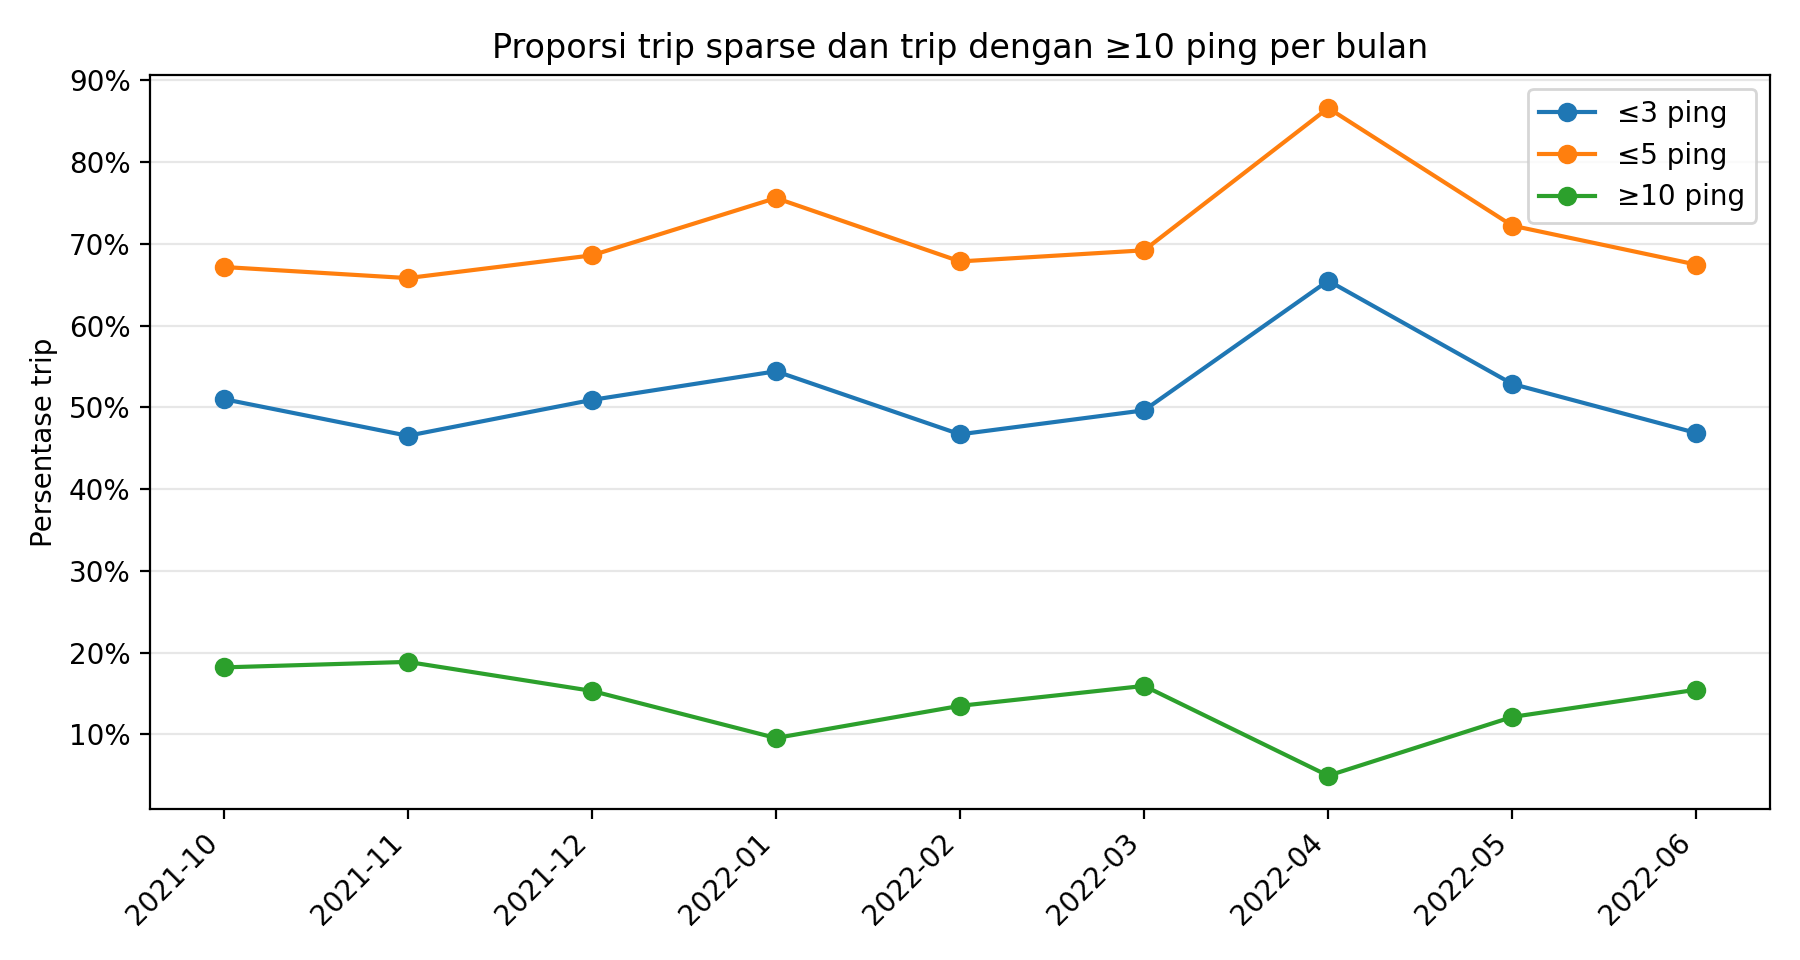
\includegraphics[width=0.95\textwidth]{../results/trip_ping_distribution/all_months_sparse_share.png}
\caption{Persentase trip sparse berdasarkan jumlah ping per trip pada setiap bulan}
\label{fig:sparse-share}
\end{figure}

Secara bulanan, pola sparsitas muncul secara konsisten. Pada seluruh bulan pengamatan, lebih dari 65\% trip memiliki paling banyak 5 ping, dengan persentase tertinggi pada April 2022. Februari 2022 merupakan bulan dengan jumlah trip terbesar, yaitu 14.919 trip dari 3.680 MAID, sehingga bulan tersebut menjadi periode dengan basis observasi paling kuat dalam dataset.

\section{Distribusi Zona Persimpangan}

Dari 212.407 ping dalam trip valid, sebanyak 86.042 ping atau 40,5\% berada dalam zona persimpangan radius 200 meter. Distribusi per persimpangan ditunjukkan pada Tabel \ref{tab:zona}.

\begin{table}[htbp]
\centering
\caption{Distribusi Ping dan MAID dalam Zona Persimpangan}
\label{tab:zona}
\begin{tabular}{lrr}
\hline
Persimpangan & Jumlah Ping & MAID Unik\\
\hline
Monjali & 21.758 & 4.454\\
Condongcatur & 21.422 & 4.475\\
UPN & 16.882 & 3.544\\
Kentungan & 11.407 & 3.217\\
Jombor & 8.147 & 2.606\\
Kronggahan & 6.426 & 2.007\\
\hline
Total & 86.042 & 7.504\\
\hline
\end{tabular}
\end{table}

Monjali dan Condongcatur memiliki jumlah ping tertinggi dan jumlah MAID unik yang hampir sama. Hal ini menunjukkan bahwa kedua simpang tersebut merupakan zona dengan intensitas pengamatan kendaraan terbesar dalam dataset. Sementara itu, Kronggahan memiliki jumlah ping dan MAID terendah, yang menunjukkan bahwa bagian barat koridor relatif lebih rendah intensitas pengamatannya dibandingkan bagian tengah dan timur.

\section{Analisis Matriks Origin-Destination}

\subsection{Matriks OD Agregat}

Dari 38.973 trip valid, sebanyak 28.767 trip memiliki pasangan origin dan destination yang teridentifikasi pada enam zona persimpangan. Matriks OD agregat ditunjukkan pada Tabel \ref{tab:od} dan divisualisasikan pada Gambar \ref{fig:od-all}.

\begin{table}[htbp]
\centering
\caption{Matriks OD Agregat Oktober 2021--Juni 2022}
\label{tab:od}
\small
\begin{tabular}{lrrrrrr}
\hline
O\textbackslash D & Kron. & Jomb. & Monj. & Kent. & Cond. & UPN\\
\hline
Kronggahan & 1.419 & 338 & 380 & 127 & 281 & 195\\
Jombor & 384 & 1.632 & 651 & 222 & 361 & 262\\
Monjali & 375 & 448 & 3.438 & 466 & 752 & 522\\
Kentungan & 151 & 148 & 585 & 2.341 & 553 & 340\\
Condongcatur & 242 & 209 & 842 & 486 & 3.765 & 956\\
UPN & 147 & 120 & 504 & 205 & 692 & 4.228\\
\hline
\end{tabular}
\end{table}

\begin{figure}[htbp]
\centering
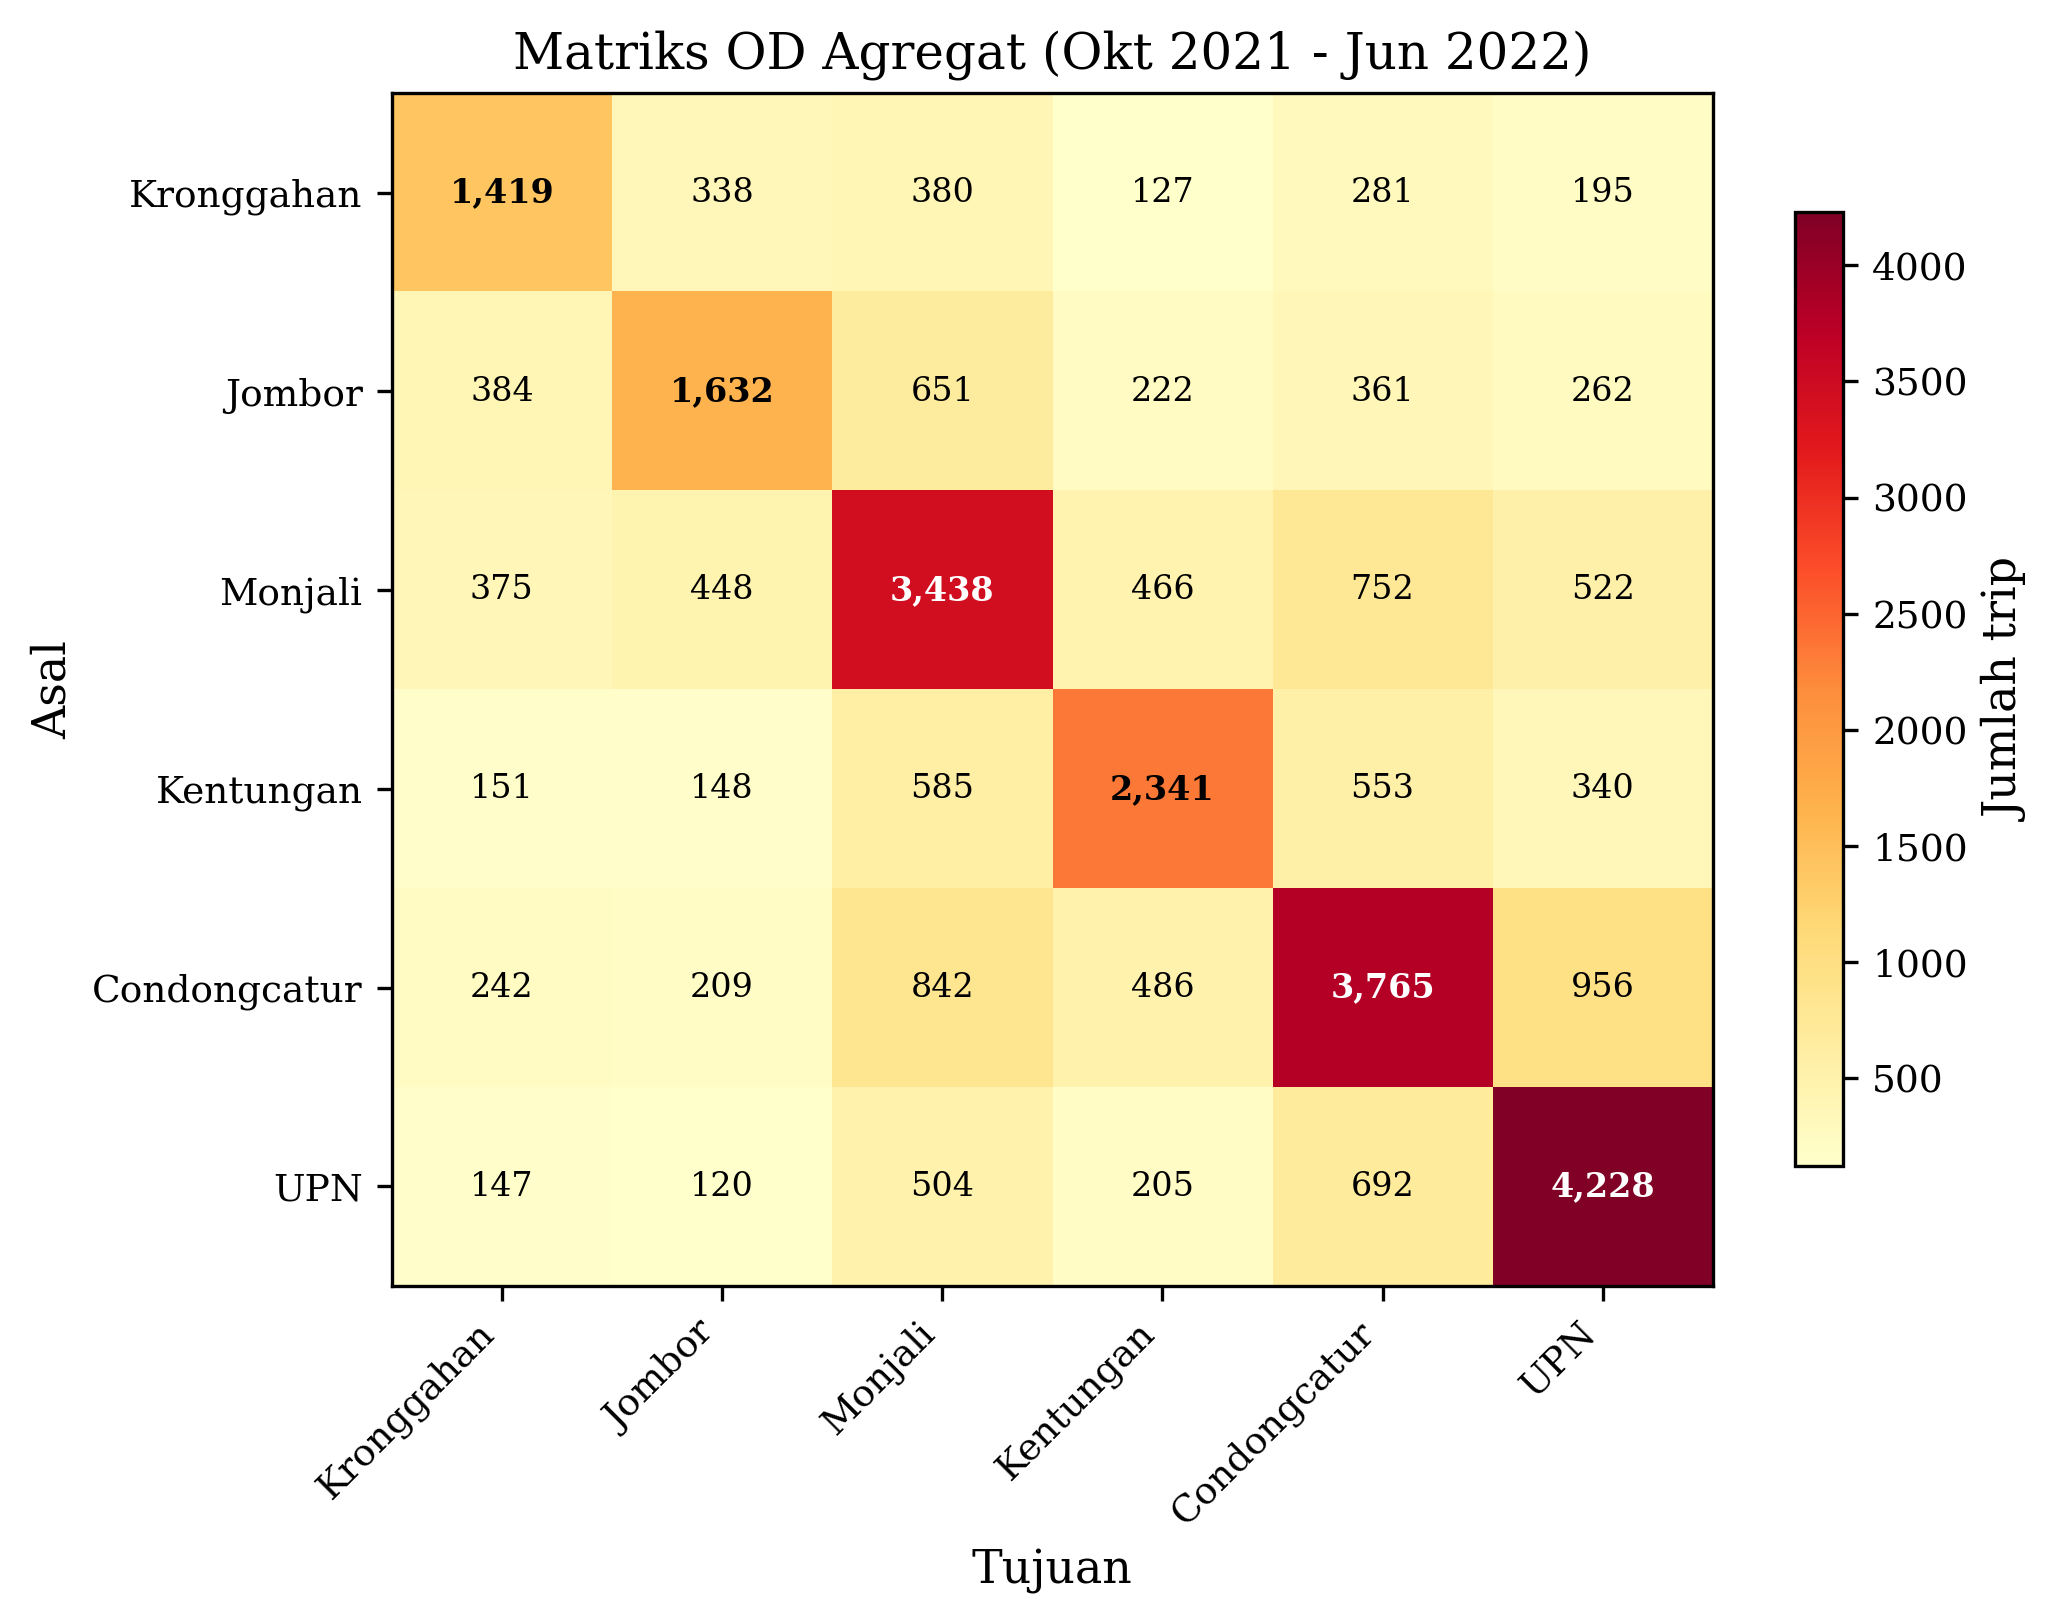
\includegraphics[width=0.85\textwidth]{../results/figures/od_matrix/od_heatmap_all.png}
\caption{Visualisasi matriks OD agregat pada enam persimpangan Ring Road Utara}
\label{fig:od-all}
\end{figure}

Total perjalanan OD teridentifikasi adalah 28.767 trip. Sebanyak 16.823 trip atau 58,48\% berada pada diagonal utama, yaitu origin dan destination terdeteksi pada zona persimpangan yang sama. Dominasi diagonal ini tidak selalu berarti kendaraan benar-benar melakukan putar balik, melainkan dapat mencerminkan trip pendek atau trip sparse yang hanya teramati pada satu zona persimpangan.

Pasangan OD non-diagonal terbesar adalah Condongcatur--UPN sebanyak 956 trip, diikuti Condongcatur--Monjali sebanyak 842 trip, Monjali--Condongcatur sebanyak 752 trip, dan UPN--Condongcatur sebanyak 692 trip. Pola ini menunjukkan kuatnya interaksi kendaraan teramati pada bagian tengah--timur koridor RRU.

\subsection{Perbandingan Hari Kerja dan Akhir Pekan}

Matriks OD hari kerja mencakup 19.833 trip atau 68,94\% dari total OD teridentifikasi. Sementara itu, akhir pekan mencakup 8.934 trip atau 31,06\%. Perbandingan ini menunjukkan bahwa jumlah absolut OD teridentifikasi lebih banyak pada hari kerja dalam sampel. Namun, karena jumlah hari kerja pada periode pengamatan lebih banyak daripada akhir pekan, interpretasi intensitas harian memerlukan normalisasi terhadap jumlah hari dan tidak cukup berdasarkan total absolut semata.

\begin{figure}[htbp]
\centering
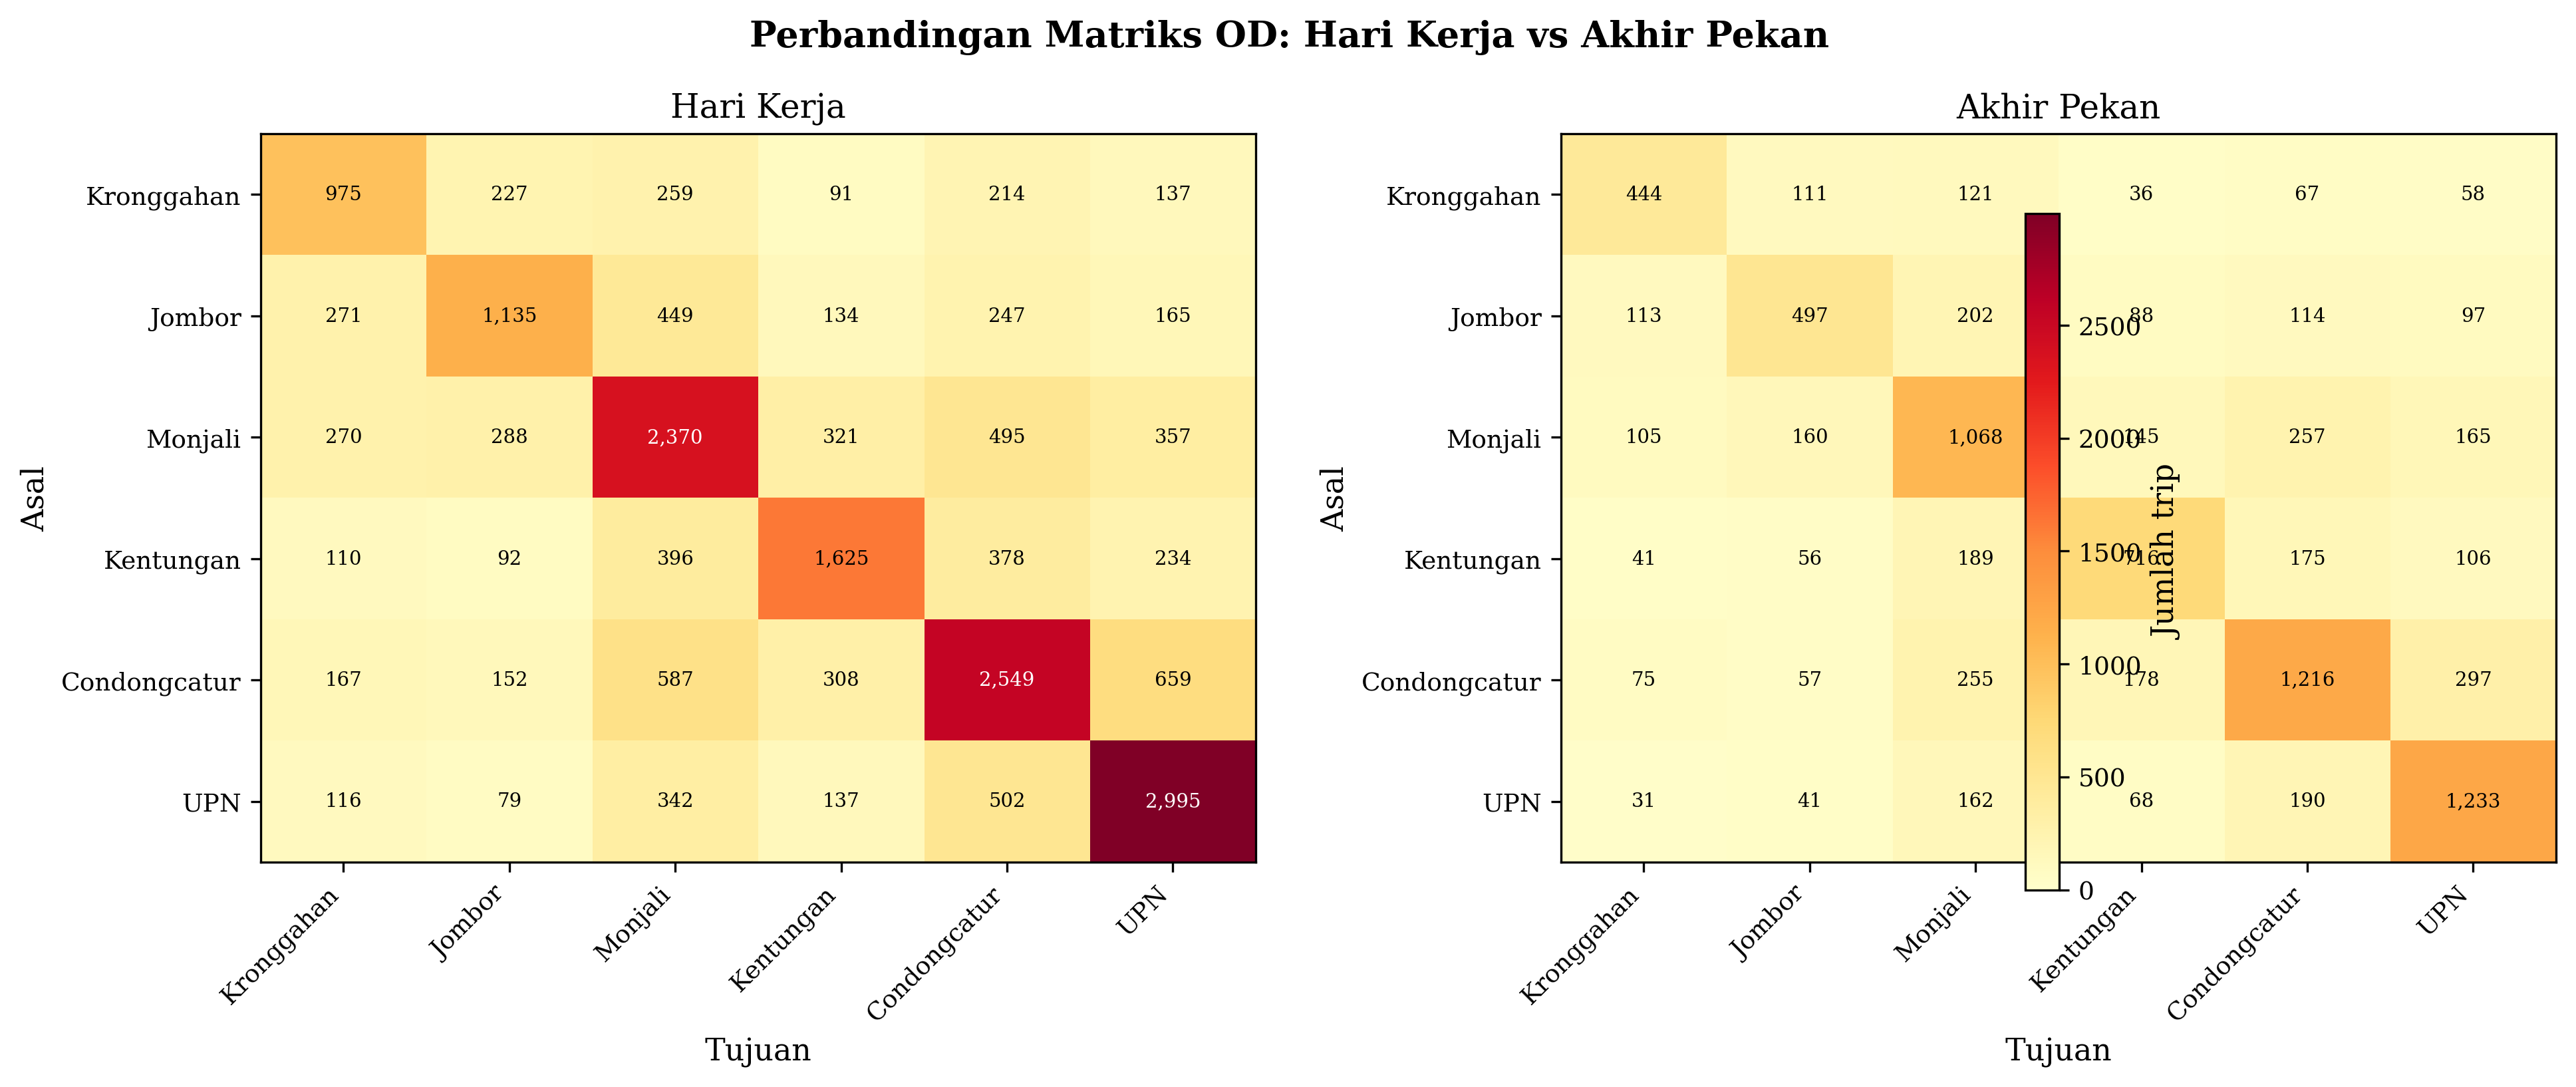
\includegraphics[width=0.95\textwidth]{../results/figures/od_matrix/od_weekday_weekend_comparison.png}
\caption{Perbandingan OD hari kerja dan akhir pekan}
\label{fig:od-weekday-weekend}
\end{figure}

\subsection{Perbandingan Jam Sibuk dan Non-Sibuk}

OD pada jam sibuk mencakup 7.121 trip atau 24,75\% dari total OD teridentifikasi. Sebaliknya, jam non-sibuk mencakup 21.646 trip atau 75,25\%. Karena definisi jam sibuk hanya mencakup empat jam per hari, jumlah absolut pada jam non-sibuk secara wajar lebih besar. Oleh karena itu, interpretasi yang lebih tepat bukan membandingkan total absolut semata, melainkan melihat konsentrasi relatif dan pola pasangan OD yang muncul pada jam sibuk.

\section{Analisis Indikator Intensitas Persimpangan}

Indikator intensitas persimpangan dihitung menggunakan MAID unik dan jumlah ping yang teramati dalam zona persimpangan. Istilah intensitas digunakan untuk menghindari klaim bahwa nilai yang dihitung merupakan kepadatan atau volume lalu lintas aktual. Ringkasan peringkat rata-rata harian berdasarkan agregasi MAID unik per hari ditunjukkan pada Tabel \ref{tab:density-rank}.

\begin{table}[htbp]
\centering
\caption{Peringkat Indikator Intensitas Rata-Rata Harian Persimpangan}
\label{tab:density-rank}
\begin{tabular}{clrr}
\hline
Peringkat & Persimpangan & Rata-rata MAID/hari & Total MAID Unik\\
\hline
1 & Condongcatur & 39,6 & 4.475\\
2 & Monjali & 39,3 & 4.454\\
3 & UPN & 30,1 & 3.544\\
4 & Kentungan & 27,6 & 3.217\\
5 & Jombor & 21,4 & 2.606\\
6 & Kronggahan & 15,6 & 2.007\\
\hline
\end{tabular}
\end{table}

Condongcatur dan Monjali menempati dua peringkat tertinggi dengan nilai rata-rata harian yang hampir sama. UPN berada pada peringkat ketiga, sedangkan Kronggahan memiliki intensitas terendah. Secara spasial, pola ini mengindikasikan bahwa bagian tengah hingga timur RRU memiliki intensitas kendaraan teramati lebih tinggi dibandingkan sisi barat dalam sampel MPD aktif.

\begin{figure}[htbp]
\centering
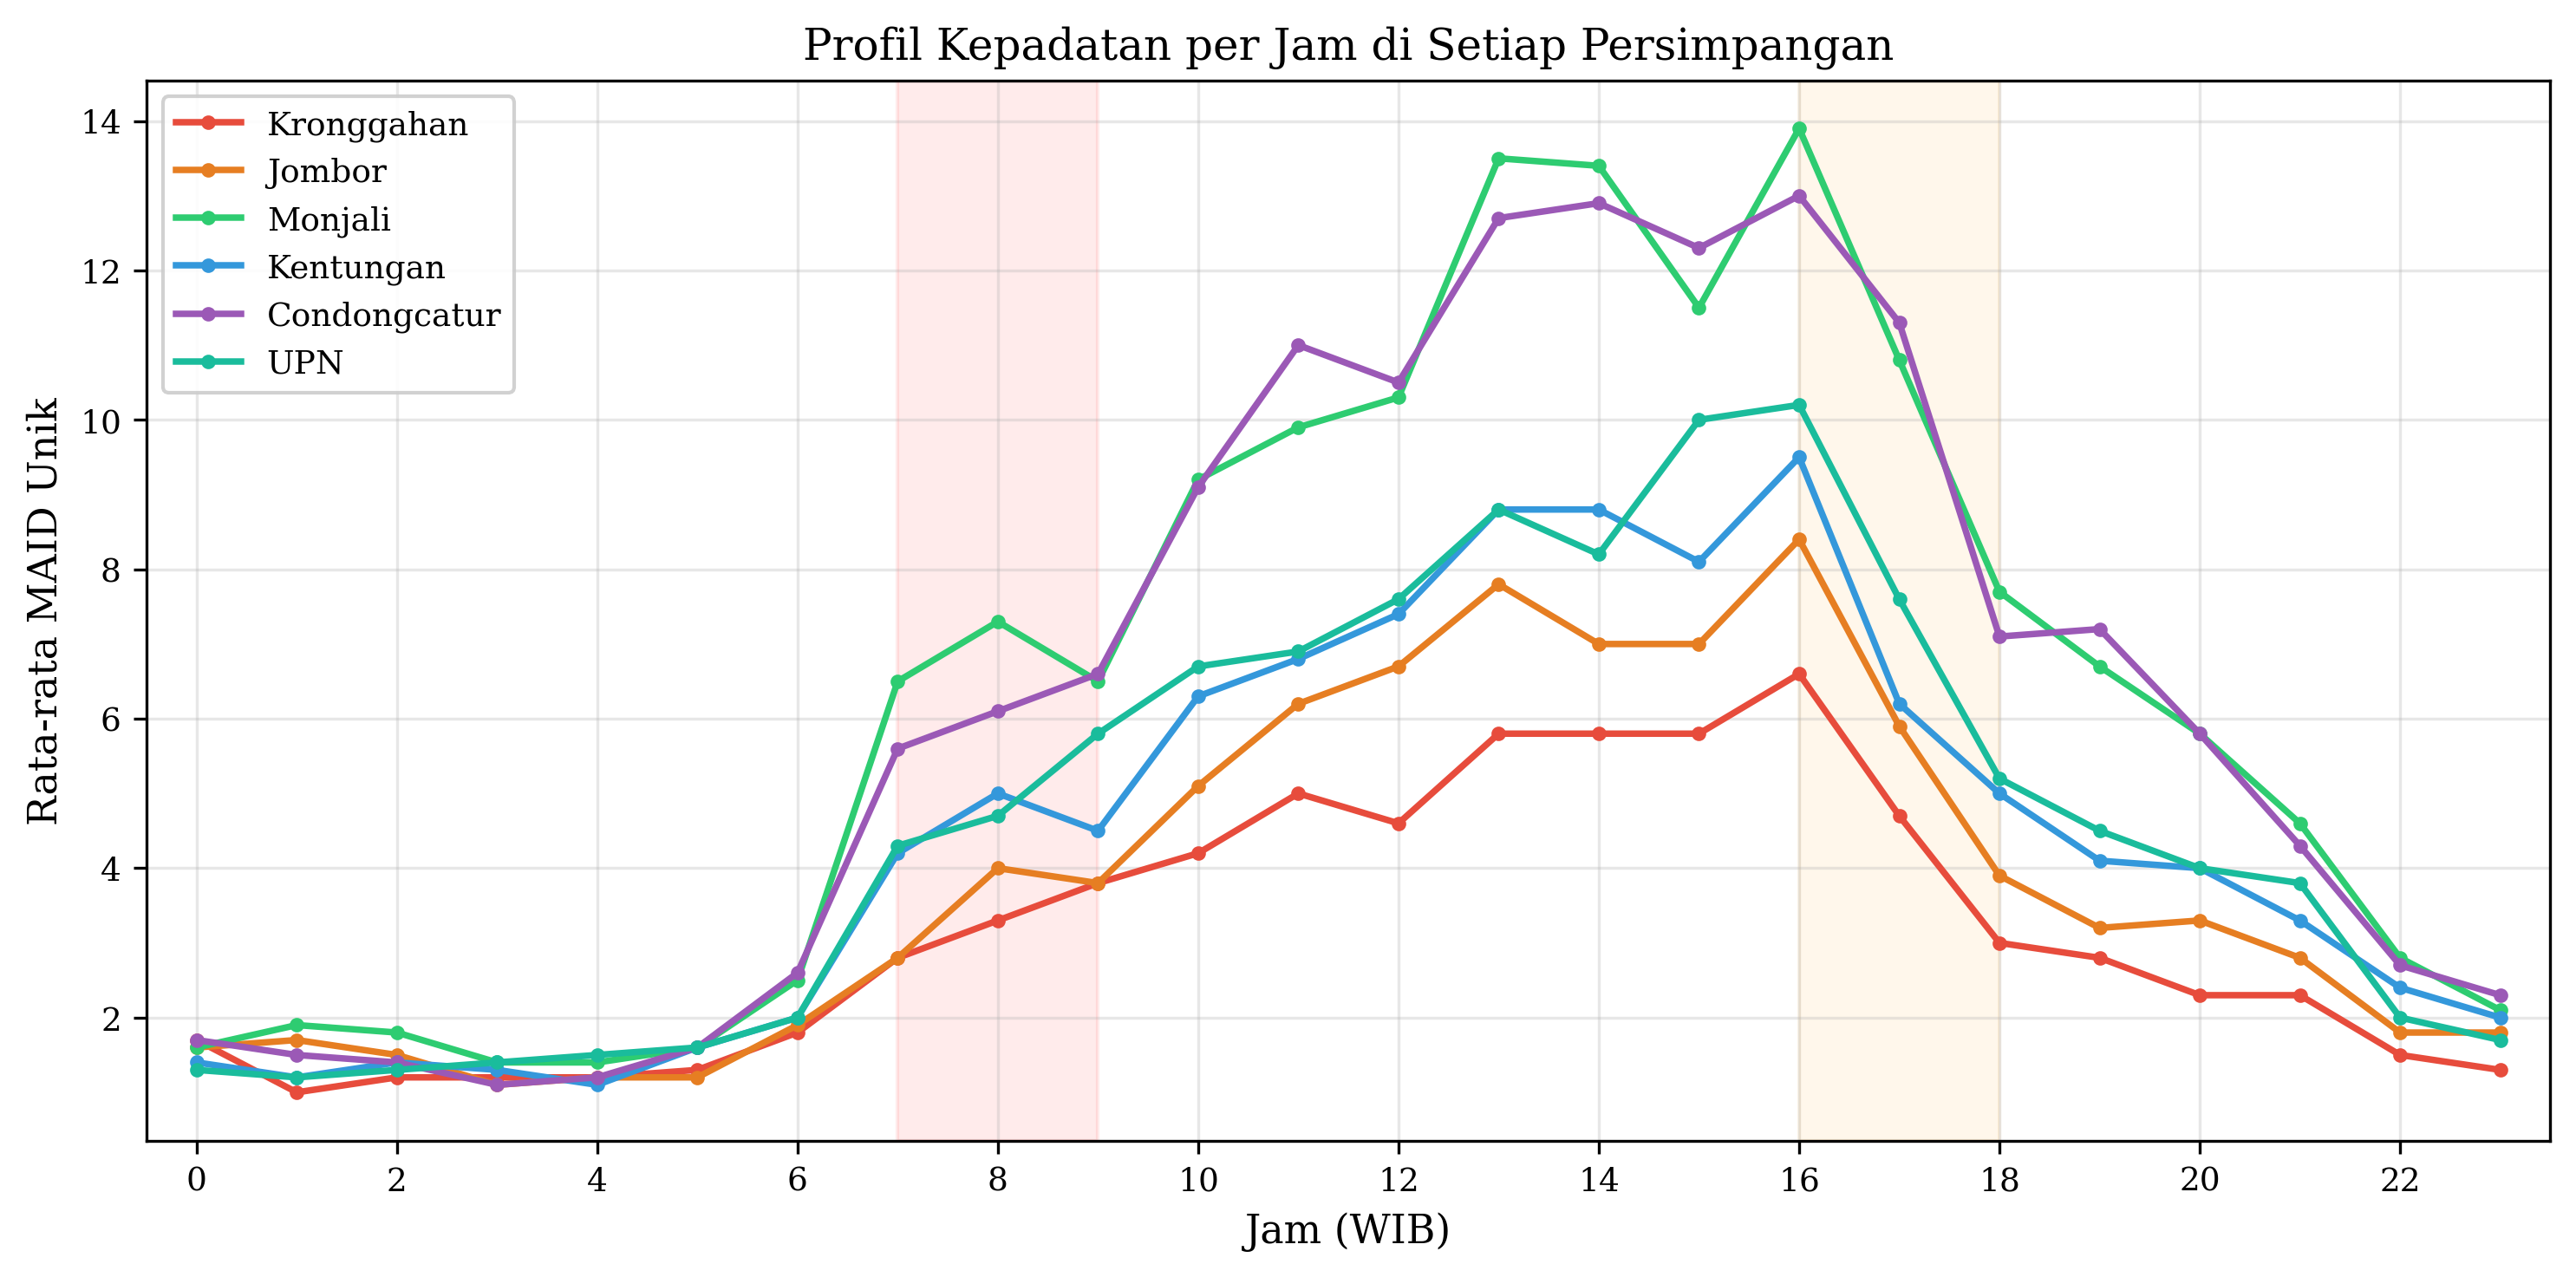
\includegraphics[width=0.95\textwidth]{../results/figures/density/density_hourly_profile.png}
\caption{Profil intensitas per jam berdasarkan rata-rata MAID unik dalam zona persimpangan}
\label{fig:density-hourly}
\end{figure}

Gambar \ref{fig:density-hourly} menunjukkan profil intensitas per jam pada seluruh persimpangan. Secara umum, intensitas meningkat pada pagi hari, tetap relatif tinggi pada periode siang hingga sore, dan menurun pada malam hari. Pola tersebut selaras dengan dugaan fungsi RRU sebagai koridor aktivitas harian perkotaan, tetapi tetap perlu dibaca sebagai pola perangkat teramati dalam sampel MPD aktif.

\begin{figure}[htbp]
\centering
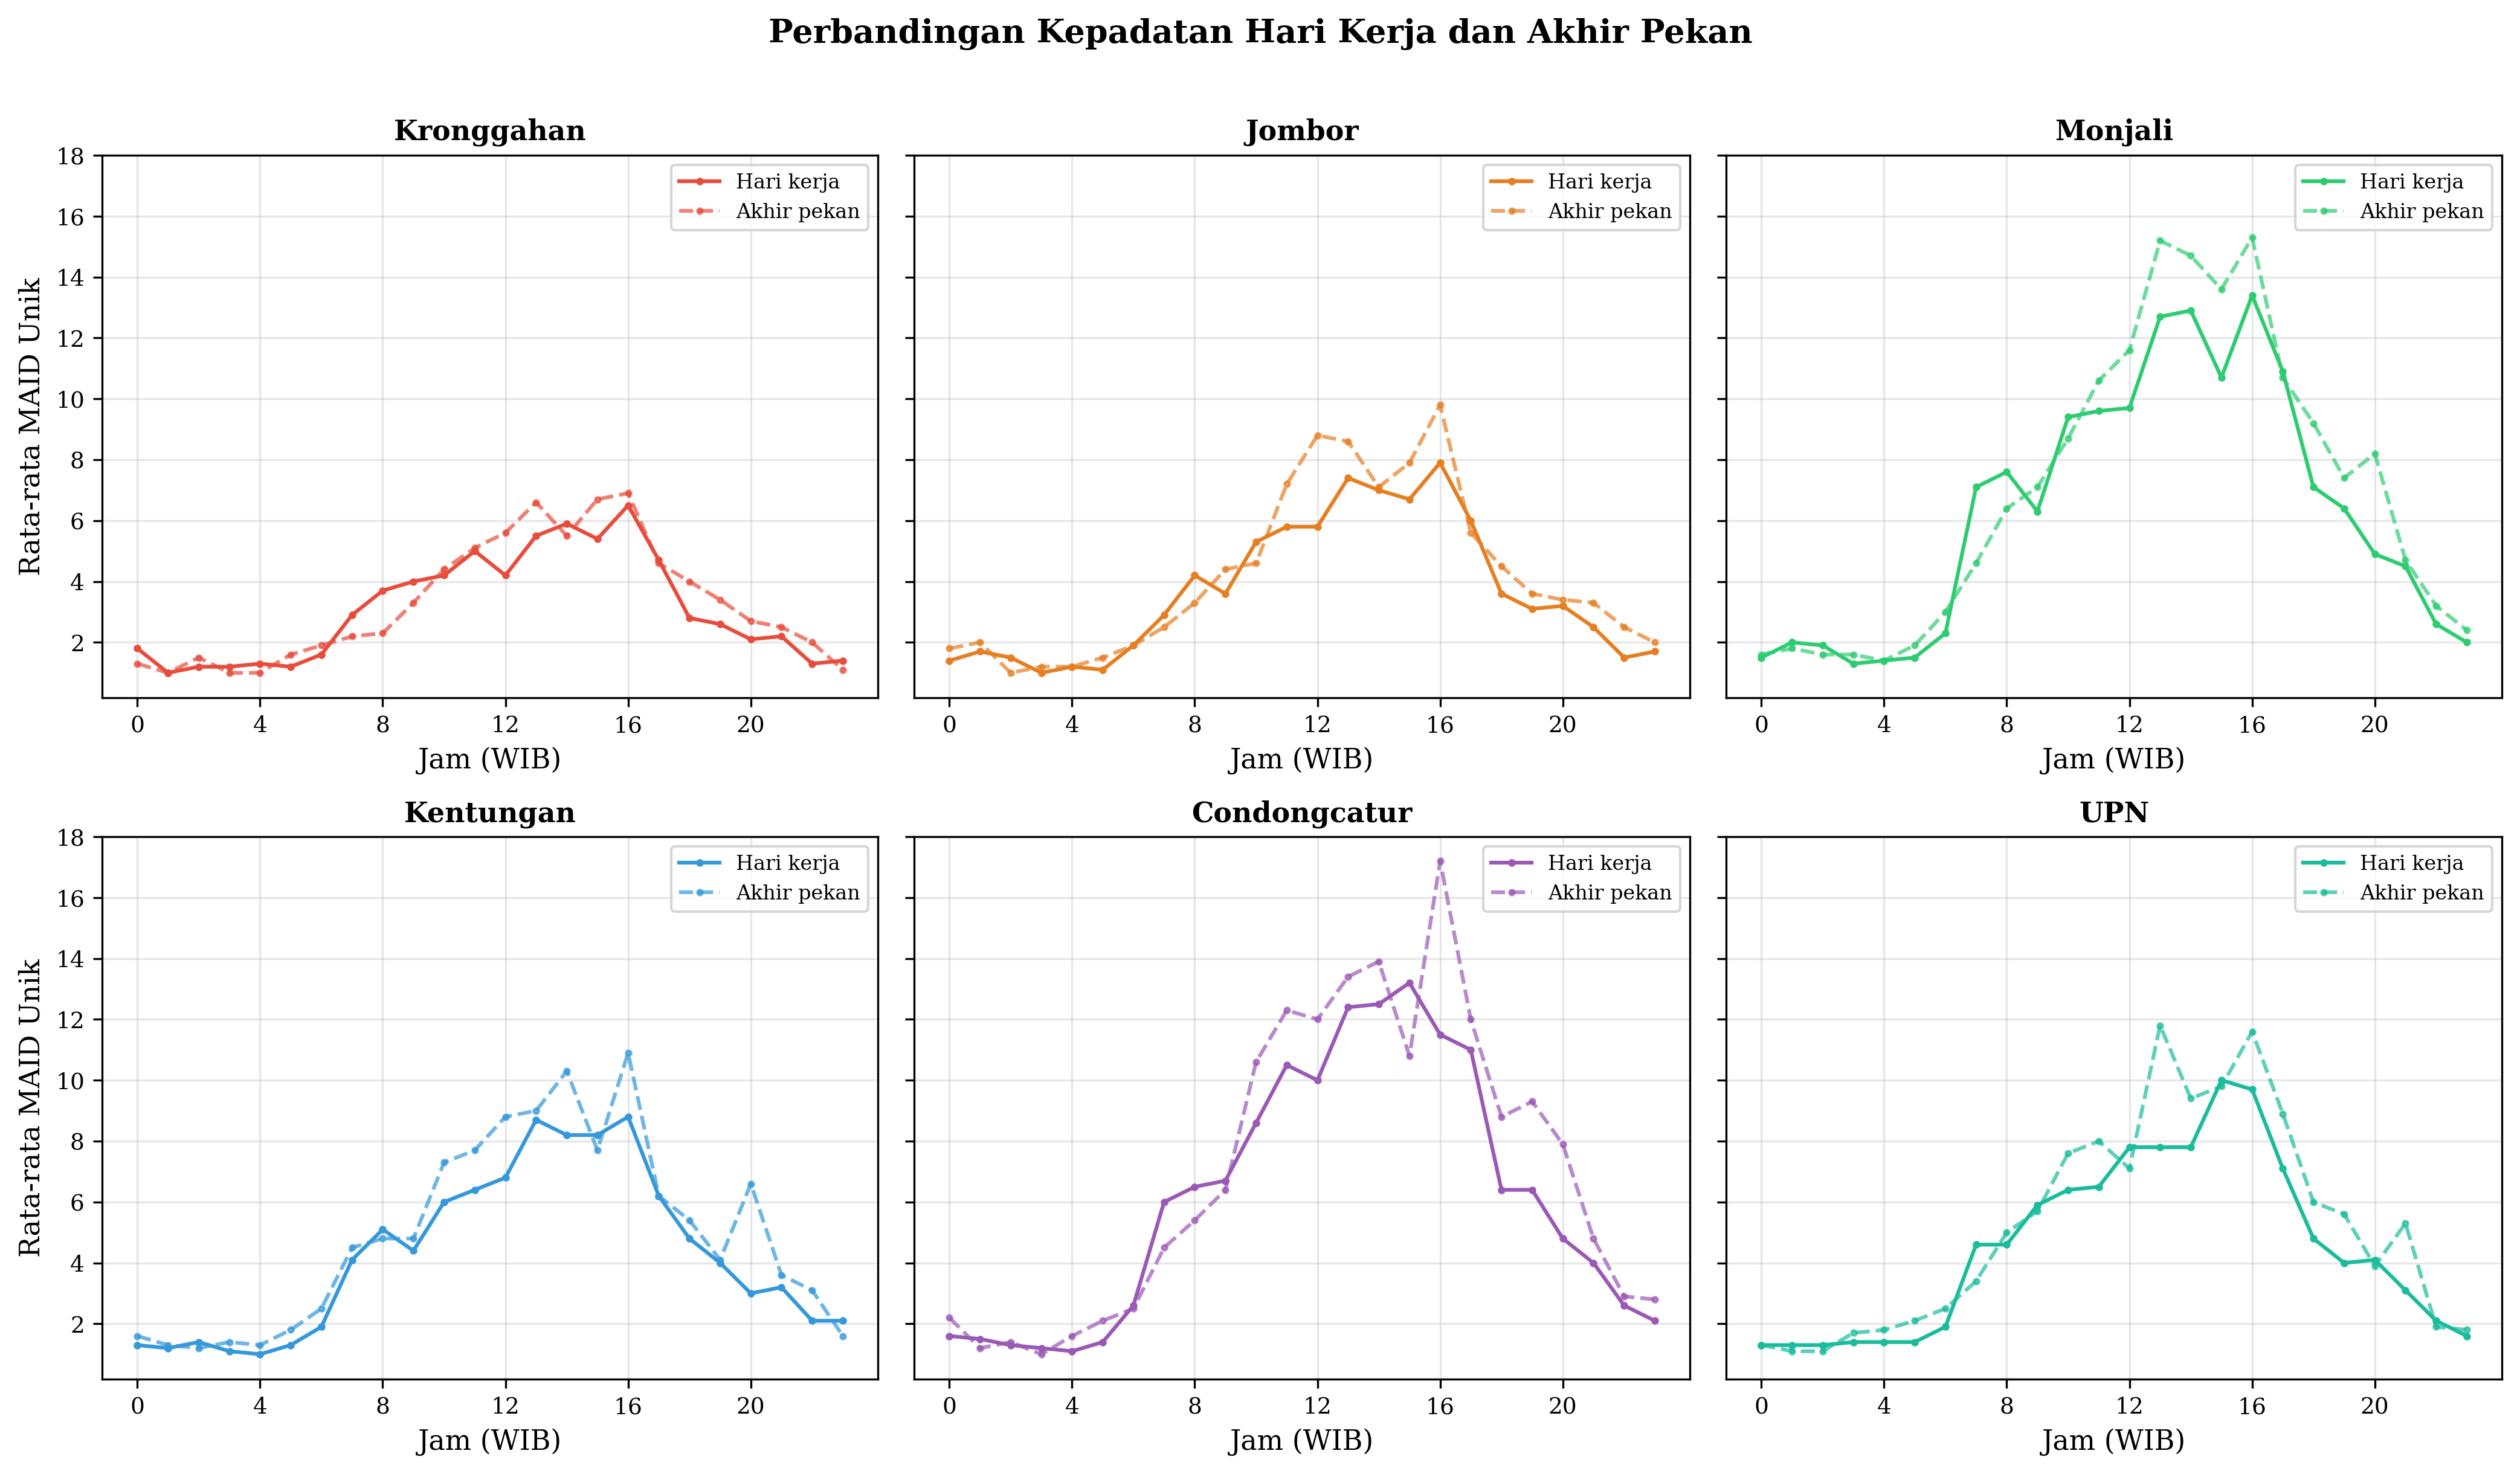
\includegraphics[width=0.95\textwidth]{../results/figures/density/density_weekday_weekend.png}
\caption{Perbandingan profil intensitas hari kerja dan akhir pekan}
\label{fig:density-weekday-weekend}
\end{figure}

Perbandingan hari kerja dan akhir pekan memperlihatkan bahwa beberapa persimpangan memiliki profil hari kerja yang lebih kuat, khususnya pada jam aktivitas. Namun, karena MPD aktif memiliki cakupan sampel yang tidak seragam, perbedaan tersebut perlu dipahami sebagai variasi intensitas perangkat teramati, bukan perubahan volume kendaraan aktual yang tervalidasi.

\section{Analisis Pola OD Zona Eksploratif}

Klasifikasi pola OD zona eksploratif mengidentifikasi 26 pola pergerakan pada enam persimpangan. Hasil lengkap divisualisasikan pada Gambar \ref{fig:turning}.

\begin{figure}[htbp]
\centering
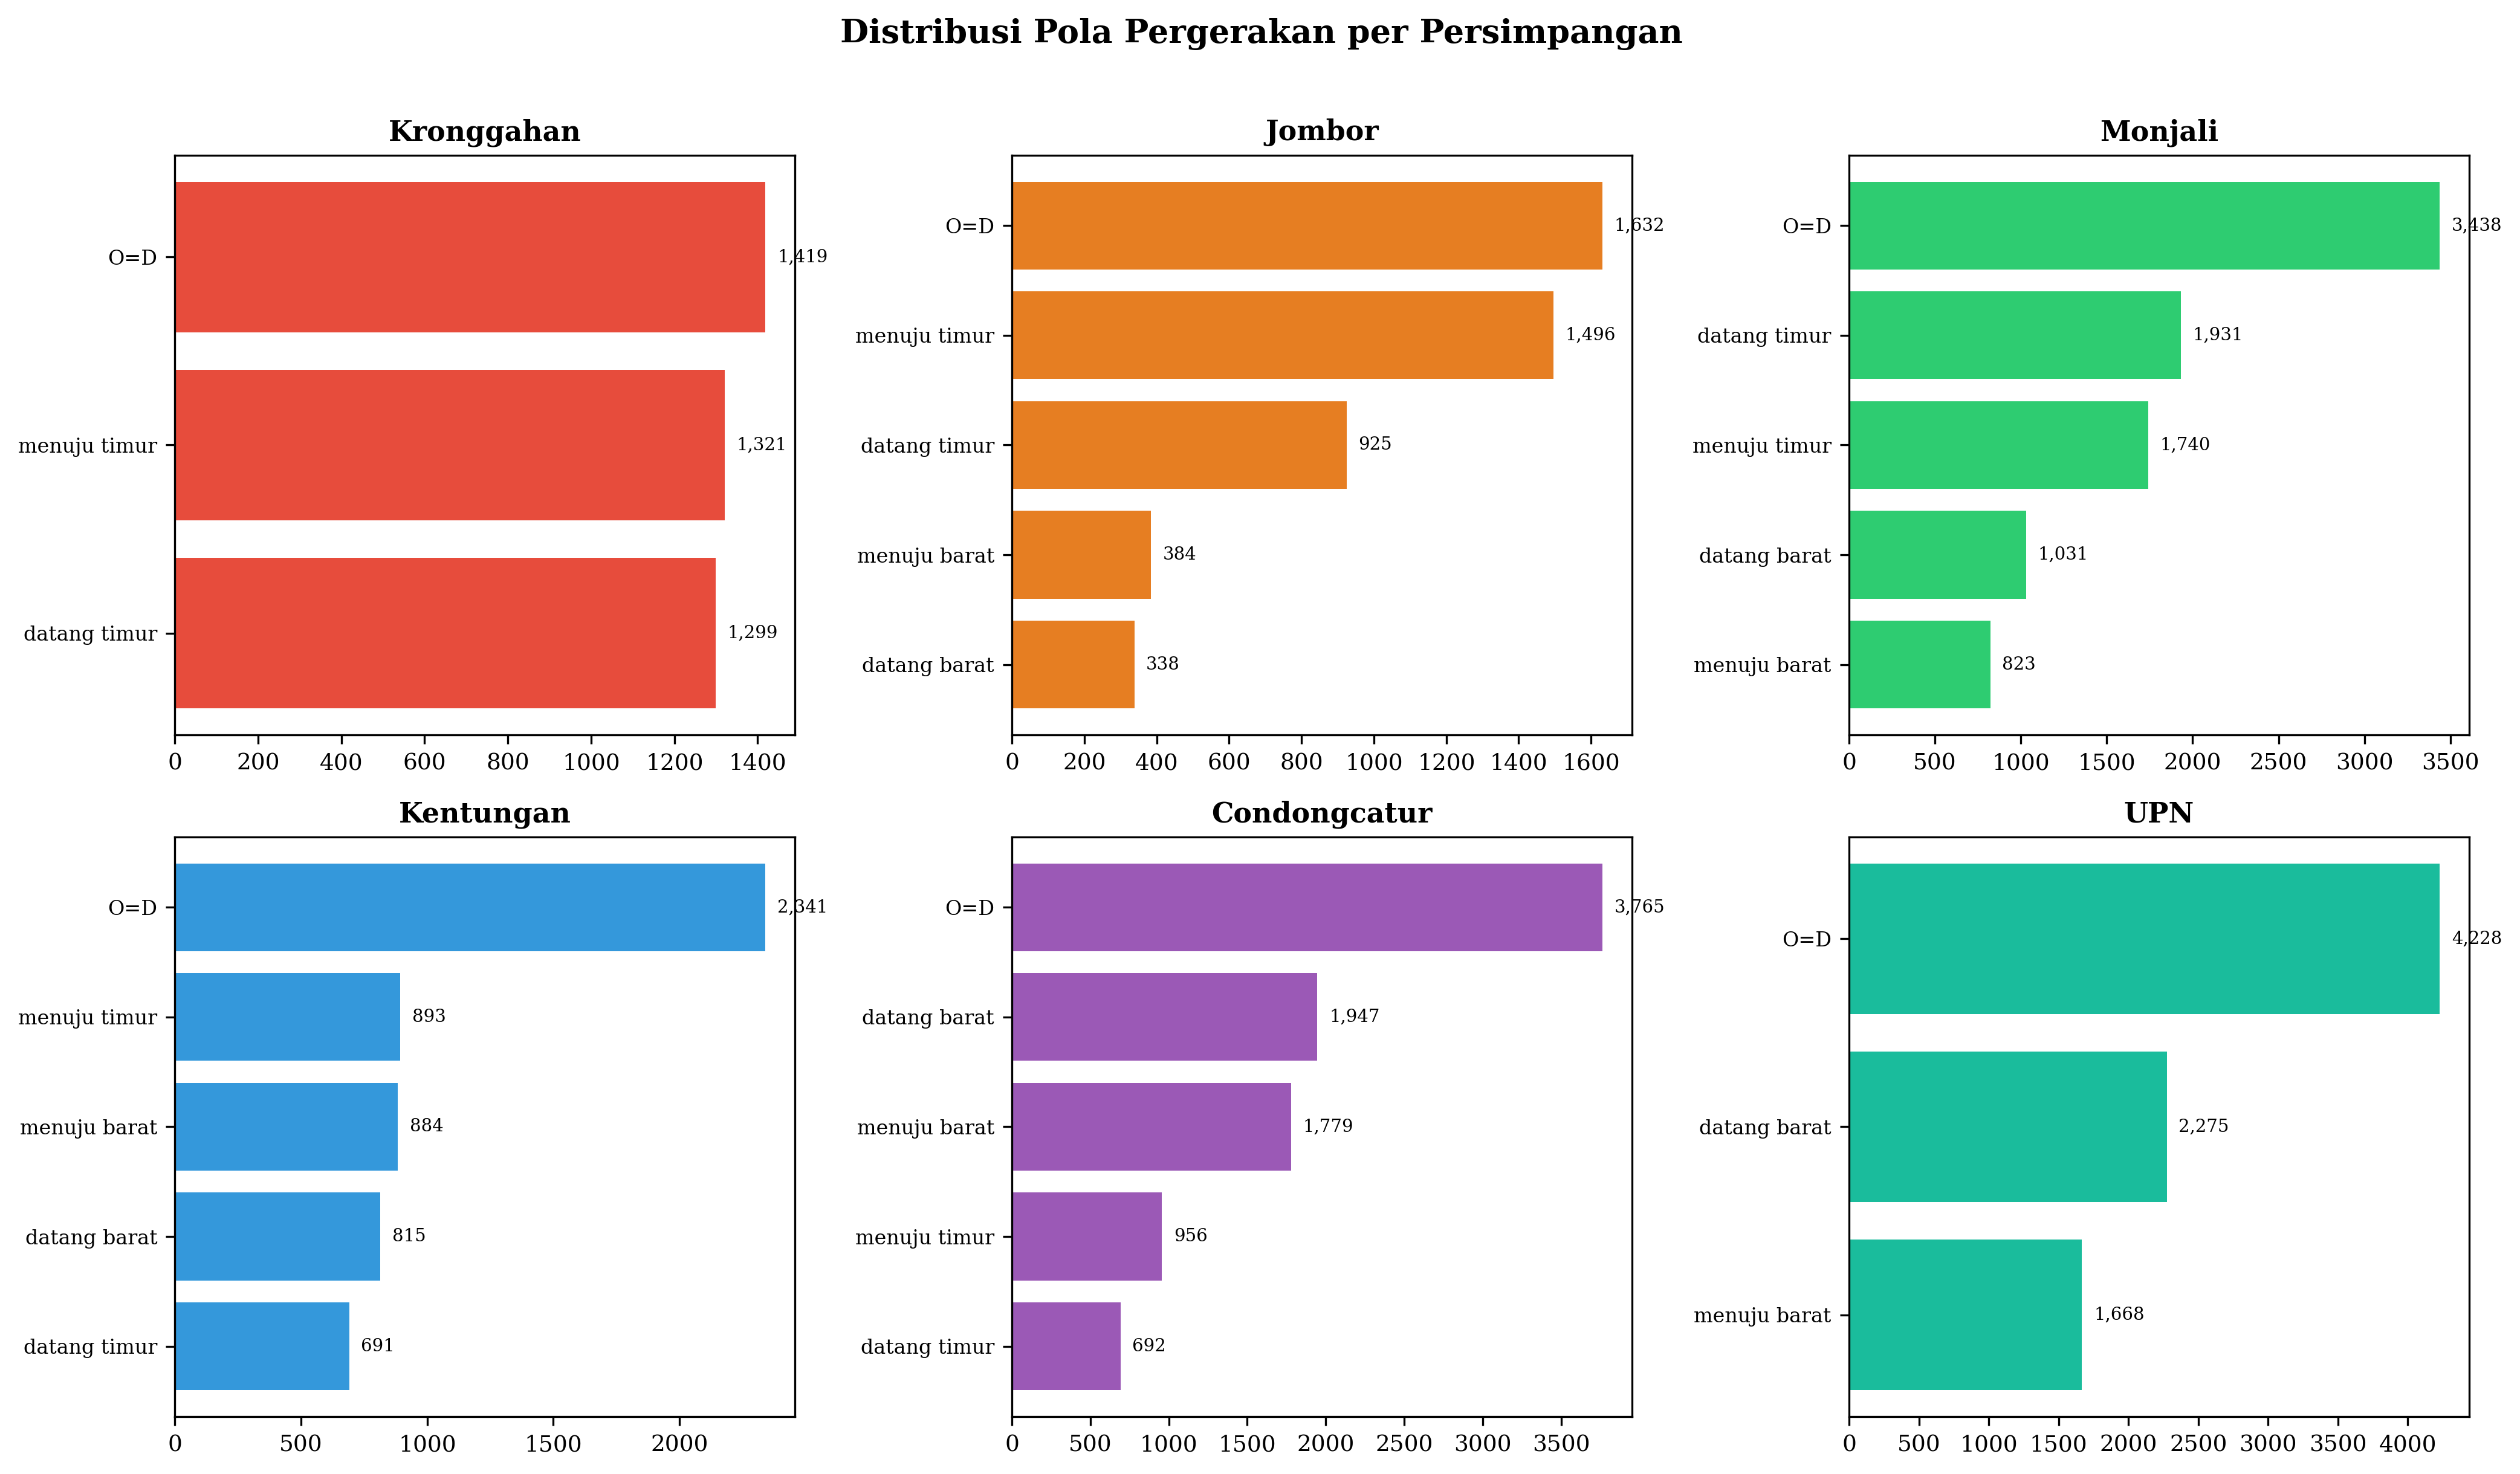
\includegraphics[width=0.95\textwidth]{../results/figures/turning_movement/turning_movements_all.png}
\caption{Distribusi pola OD zona eksploratif per persimpangan}
\label{fig:turning}
\end{figure}

Secara agregat, kategori terbesar adalah O=D atau zona sama sebanyak 16.823 pola. Dalam konteks penelitian ini, kategori tersebut tidak ditafsirkan sebagai putar balik fisik di simpang. Kategori ini terutama menunjukkan trip dengan origin dan destination pada zona yang sama. Kondisi tersebut dapat terjadi karena trip pendek, kendaraan hanya teramati pada satu zona persimpangan, atau frekuensi pencuplikan GPS yang rendah.

Kategori berikutnya adalah indikasi kedatangan dari barat dan keberangkatan ke timur, masing-masing sebanyak 6.406 pola, serta keberangkatan ke barat dan kedatangan dari timur, masing-masing sebanyak 5.538 pola. Pola tersebut menunjukkan adanya indikasi pergerakan sepanjang koridor barat--timur dan timur--barat, tetapi hasilnya tetap harus dibaca sebagai klasifikasi zona berbasis OD, bukan observasi geometris belokan aktual.

\section{Pembahasan}

\subsection{Makna Hasil sebagai Baseline Spatiotemporal}

Hasil penelitian menunjukkan bahwa MPD aktif dapat dimanfaatkan untuk menyusun \textit{baseline} deskriptif kendaraan terindikasi pada koridor Ring Road Utara. Baseline tersebut mencakup tiga informasi utama. Pertama, matriks OD zona memberikan gambaran pasangan persimpangan yang paling sering muncul dalam trip teramati. Kedua, indikator intensitas persimpangan menunjukkan perbedaan kekuatan observasi antarzona, terutama tingginya intensitas di Monjali, Condongcatur, dan UPN. Ketiga, distribusi ping per trip menunjukkan batas interpretasi data sehingga analisis detail lintasan perlu dibatasi.

Dalam konteks rencana pembangunan Tol Yogyakarta--Solo, hasil ini dapat digunakan sebagai gambaran kondisi dasar sebelum perubahan jaringan jalan berdampak pada pola pergerakan permukaan. Namun, penelitian ini tidak mengklaim dampak tol secara kausal karena data yang digunakan hanya menggambarkan periode sebelum atau selama tahap awal pembangunan dan tidak mencakup kondisi setelah tol beroperasi penuh.

\subsection{Keterbatasan Interpretasi}

Keterbatasan utama penelitian ini adalah sifat data MPD aktif yang sparse dan berbasis sampel. Mayoritas trip hanya memiliki sedikit titik observasi, sehingga urutan lintasan antarping tidak dapat direkonstruksi secara detail. Selain itu, data hanya mencakup perangkat yang mengaktifkan layanan lokasi dan termasuk dalam cakupan penyedia data. Oleh karena itu, jumlah ping, MAID, dan trip tidak boleh disamakan dengan volume lalu lintas aktual.

Dengan pembatasan tersebut, hasil penelitian diarahkan pada karakteristik perjalanan yang benar-benar teramati di koridor RRU dan tidak memperluas interpretasi ke asal perjalanan pengguna di luar koridor.
